\documentclass{article}
\usepackage{tikz}
\usetikzlibrary{shapes.geometric}
\begin{document}

\begin{figure}[h]
\centering
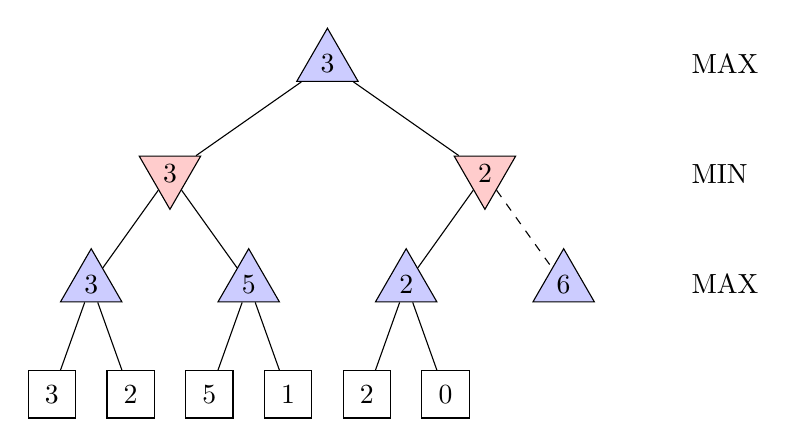
\begin{tikzpicture}[
  max/.style={regular polygon, regular polygon sides=3, draw, fill=blue!20, inner sep=1pt, minimum size=9mm},
  min/.style={regular polygon, regular polygon sides=3, shape border rotate=180, draw, fill=red!20, inner sep=1pt, minimum size=9mm},
  leaf/.style={rectangle, draw, minimum size=6mm},
  level 1/.style={sibling distance=40mm},
  level 2/.style={sibling distance=20mm},
  level 3/.style={sibling distance=10mm},
  level distance=14mm
]
\node[max] {3}
  child {node[min] {3}
    child {node[max] {3}
      child {node[leaf] {3}}
      child {node[leaf] {2}}
    }
    child {node[max] {5}
      child {node[leaf] {5}}
      child {node[leaf] {1}}
    }
  }
  child {node[min] {2}
    child {node[max] {2}
      child {node[leaf] {2}}
      child {node[leaf] {0}}
    }
    child {node[max] {6} edge from parent[dashed]
    }
  };
\node[anchor=west] at (4.5,0) {MAX};
\node[anchor=west] at (4.5,-1.4) {MIN};
\node[anchor=west] at (4.5,-2.8) {MAX};
\end{tikzpicture}
\caption{Minimax with alpha-beta pruning; the dashed branch is pruned.}
\end{figure}

\end{document}
